
\chapter{Dancing Links}
\label{dancing_links}

Dancing Links (DLX) is an algorithm invented by Donald Knuth to solve any exact cover problem.
It was first described in \cite{knuth00dancing} where he looks at the details of the algorithm and uses it to solve some practical problems.
Before we look at the DLX algorithm in more detail we need to explain what an exact cover problem is.



\section{Exact cover}
\label{exact_cover}

To represent an exact cover problem we use a matrix in which each element is either zero or one (non-zero).
This type of matrix is called a boolean, binary, logical or \{0,1\}-matrix.
We use ``matrix'' in the rest of this report to mean a boolean matrix and to prevent ambiguity ``non-zero'' is used instead of ``one'' to identify the value of a matrix element\footnote{A non-zero value is effectively the same as one because a boolean matrix can only have elements zero and one.}.

\begin{definition}
Given a collection of subsets $E$ of a set $U$, an exact cover is a subset $S$ of $E$ such that each element of $U$ appears once in $S$.
\end{definition}

The set $U$ is the set of columns $U = \{ 1, 2, \ldots, n \}$.
$E$ is the collection of rows where each set contains the number of the columns which has non-zero values.
The idea is that each column in the matrix represents a specific constraint and each row is a way to satisfy some of the constraints.

For the general $m \times n$ matrix
\[
A =
\left[
\begin{array}{ccccc}
	a_{1,1} & a_{1,2} & a_{1,3} & \cdots & a_{1,n} \\
	a_{2,1} & a_{2,2} & a_{2,3} & \cdots & a_{2,n} \\
	a_{3,1} & a_{3,2} & a_{3,3} & \cdots & a_{3,n} \\
	\vdots  & \vdots  & \vdots  & \ddots & \vdots  \\
	a_{m,1} & a_{m,2} & a_{m,3} & \cdots & a_{m,n} \\
\end{array}
\right]
\]
$a_{i,j}$ is an element in the matrix at row $i$, column $j$ where $a_{i,j} \in \{0,1\}$.
The number of rows is $m$ and the number of columns is $n$.
A subset of rows from a matrix is an exact cover iff (if and only if) each column has exactly one non-zero (one) element.
Let $R_A$ and $R_B$ be the set of rows in matrix $A$ and $B$ respectively.
If $R_B \subseteq R_A$ then $B$ forms the following $k \times n$ matrix
\[
	B =
	\left[
	\begin{array}{ccccc}
		b_{1,1} & b_{1,2} & b_{1,3} & \cdots & b_{1,n} \\
		b_{2,1} & b_{2,2} & b_{2,3} & \cdots & b_{2,n} \\
		b_{3,1} & b_{3,2} & b_{3,3} & \cdots & b_{3,n} \\
		\vdots  & \vdots  & \vdots  & \ddots & \vdots  \\
		b_{k,1} & b_{k,2} & b_{k,3} & \cdots & b_{k,n} \\
	\end{array}
	\right]
\]
$k \leq m$ so that $B$ is a reduced matrix of $A$ or, in the case where $k = m$, the two matrices are identical.
The number of columns in $A$ and $B$ is always the same.
The subset $R_B$ is an exact cover iff the following equation is satisfied
\[
	\sum_{i = 1}^{k} b_{i,j} = 1 \;\;\; \text{for all } j \in \{ 1, 2, \ldots, n \}
\]

\begin{example}
In practical applications we are usually given an initial matrix $A$ and tasked with finding all the subsets of rows which are exact covers.
For example the following matrix
\begin{equation}
	\left[
	\begin{array}{cccc}
		1 & 0 & 0 & 0 \\
		0 & 1 & 1 & 0 \\
		1 & 0 & 0 & 1 \\
		0 & 0 & 1 & 1 \\
		0 & 1 & 0 & 0 \\
		0 & 0 & 1 & 0 \\
	\end{array}
	\right]
	\label{eq:cover_example}
\end{equation}
represents a specific exact cover problem.
In this matrix row 2 and 3 form a valid solution (exact cover) because the subset of rows $\{ 2, 3 \}$, and thus the reduced matrix
\[
\left[
\begin{array}{cccc}
	0 & 1 & 1 & 0 \\
	1 & 0 & 0 & 1 \\
\end{array}
\right]
\]
has exactly one non-zero element in each column.
By adopting a trial and error approach one can find that the full set of solutions for the matrix in (\ref{eq:cover_example}) is $\{ \{1, 4, 5 \}, \{ 2, 3\}, \{ 3, 5, 6\} \}$.
\end{example}


\subsection{Generalized exact cover}

A generalized form of the exact cover problem is sometimes better suited to solve certain types of problems.
The generalized problem can be translated to an exact cover problem by adding additional rows, but translating in the opposite direction is not always possible.
The generalized problem divides the matrix into primary and secondary columns which are subject to two different sets of constraints.
Each primary column in the solution must have exactly one non-zero element, as before.
However, each secondary column in the solution can have either zero or one non-zero element, instead of exactly one.

Let $C_P$ be the set of primary columns and $C_S$ the set of secondary columns in matrix $A$ and $B$.
The subset of rows $R_B$ is an exact cover iff both of the following equations are satisfied
\[
	\sum_{i = 1}^{k} b_{i,j} = 1 \;\;\; \forall j \in C_P  \;\;\;\; \wedge \;\;\;\;  \sum_{i = 1}^{k} b_{i,j} \leq 1 \;\;\; \forall j \in C_S
\]


$n$-queens (see Section \ref{queens_trans}) is one type of problem the generalized cover problem can be applied to.
Creating a secondary column for each diagonal on the chess board will reduce the number of rows in the final matrix.
Given a smaller matrix the DLX algorithm will have to do less processing to find the solutions which results in better performance.
The DLX algorithm itself does not require any modifications to solve generalized cover problems, but the matrix construction procedure requires some minor adjustments (see Section \ref{matrix_construction}).

\begin{example}
In the 4-queens problem each of the four ranks (rows) and four files (columns) on the board corresponds to a primary column in the exact cover matrix.
Each rank and file can only contain one queen, otherwise the queens would attack each other either horizontally or vertically in that rank or file.
Placing 4 queens on a $4 \times 4$ board means that each rank and file must contain exactly one queen.
However, queens can also attack diagonally, but the number of diagonals is larger than the number of queens.
The solution to the 8-queens problem in Figure \ref{fig:8queens} clearly shows that several of the diagonals have no queens.
To model this part of the problem we can use the generalized form of the exact cover problem and assign each diagonal to a secondary column.

Primary columns 1 to 4 represents the ranks 1 through 4, and primary columns 5 to 8 represents the files A to D.
On a $4 \times 4$ board there are ten diagonals if we ignore each of the four corners diagonals, which has only a single square.
The way each diagonal is numbered is unimportant as they are only needed to represent the problem and are not required in order to interpret the final solutions.
We assign each of the ten diagonals to the secondary columns 9 to 18.
Following the exact cover definition the set $U$ is the set of columns $U = \{ 1, 2, \ldots, 18 \}$.
$E$ is the collection of rows where each set contains the column numbers with non-zero elements in that row.
\begin{align*}
C =& \{ \{ 1, 5, 16 \}, \{ 1, 6, 9, 17 \}, \{ 1, 7, 10, 18 \}, \{ 1, 8, 11 \}, \\
&\{ 2, 5, 9, 15 \}, \{ 2, 6, 10, 16 \}, \{ 2, 7, 11, 17 \}, \{ 2, 8, 12, 18 \}, \\
&\{ 3, 5, 10, 14 \}, \{ 3, 6, 11, 15 \}, \{ 3, 7, 12, 16 \}, \{ 3, 8, 13, 17 \}, \\
&\{ 4, 5, 11 \}, \{ 4, 6, 12, 14 \}, \{ 4, 7, 13, 15 \}, \{ 4, 8, 16 \} \}
\end{align*}

Running this though the DLX algorithm provides two solutions $S_1$ and $S_2$.
%Notice that in each of the solutions the numbers 1 through 8, which is the primary columns, are present exactly once.
%Only eight out of the ten secondary columns are present in the solutions.
Using the first two numbers in each set (the rank and file) we can find out what the solutions look like.
Figure \ref{fig:4queens} shows the board layout of the two solutions.
\begin{align*}
S_1 = \{ \{ 1, 7, 10, 18 \}, \{ 2, 5, 9, 15 \}, \{ 3, 8, 13, 17 \}, \{ 4, 6, 12, 14 \}  \}	\\
S_2 = \{ \{ 1, 6, 9, 17 \}, \{ 2, 8, 12, 18 \}, \{ 3, 5, 10, 14 \}, \{ 4, 7, 13, 15 \}  \}	\\
\end{align*}

\begin{figure}[hptb]
	\centering 
	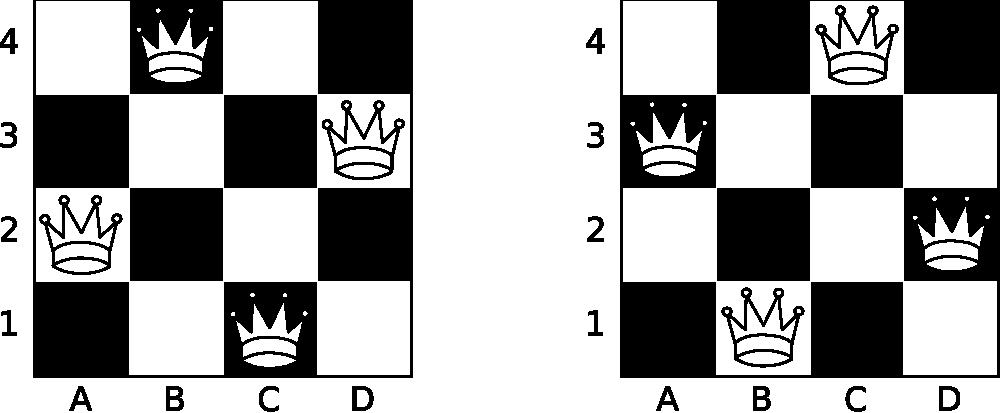
\includegraphics[width=0.44\textwidth]{queens-4x4.pdf}
	\caption{The two solutions $S_1$ (left) and $S_2$ (right) to the 4-queens problem}
	\label{fig:4queens}
\end{figure}

\end{example}



\section{Algorithm X}
\label{algox}

Exact cover is a type of problem known to be NP-complete \cite{np-comp-theory}.
Several methods exist to find all the solutions to an exact cover problem.
To find all the solutions to an exact cover problem the most straight forward algorithm is to check all possible sets of rows.
Given a set we then check to see if there is exactly one non-zero element in each column.
However, as the size of the matrix increases we will experience a combinatorial explosion on the number of possible sets to test.
The exact number of sets is $2^{m}-1$ given a matrix with $m$ rows.
The 8-queens problem (see Section \ref{queens_trans}) which has a matrix consisting of 63 rows, gives an immense 9~223~372~036~854~775~808 sets.
Given that only 92 of these are valid solutions this simple algorithm can hardly be recommended.
However, in \cite{oltean-2007} Mihai Oltean and Oana Muntean proposes a design for an optical device which should be able to solve some exact cover problems using this technique.

Another approach, which is presented in \cite{knuth00dancing}, is Algorithm X (for the lack of a better name).
This backtrack algorithm uses a more intelligent elimination method to ``wriggle'' its way through the matrix and find all the solutions.
Looking at matrix (\ref{eq:cover_example}) we can easily determine that row 1 and 3 can never be in the same set.
They are in conflict with each other because both of them have a non-zero element in the first column.
Since there must be exactly one non-zero element in each column we can rule out any set containing both row 1 and 3.

Algorithm X uses similar logic to recursively traverse the search tree by backtracking.
Backtracking is the process of exploring all possible paths in a search tree to locate solutions.
When a path in the search does not yield any solutions the algorithm backtracks and starts searching the next available path in the tree.
A modified version of Algorithm X is presented in Algorithm \ref{alg:algox}.
Changes are made to improve the readability, logical consistency and to make it easier to compare with the Dancing Links algorithm.
Algorithm X is initially called with the matrix $A$ and the column header list $H$.
$H$ is initialized with the numbers $1, 2, \ldots, n$, where $n$ is the number of columns in $A$.

\begin{algorithm}[htbp]
	\caption{Algorithm X recursive search procedure.}
	\label{alg:algox}
	\begin{distribalgo}[1]
		\PROCEDURE{search($A, H$)}
			\IF{$H$ is empty}
				\STATE Print solution and return.  \COMMENT{Base case for the recursion}
			\ENDIF
			\STATE Choose a column $c$.
			\FOREACH{row $r$ such that $a_{r,c} = 1$}
				\STATE Add $r$ to partial solution.
				\STATE Save state of matrix $A$ and list $H$.
				\FOREACH{column $j$ such that $a_{r,j} = 1$}
					\FOREACH{row $i$ such that $a_{i,j} = 1$, \textbf{except} $i = r$}
						\STATE Delete row $i$ from matrix $A$.
					\ENDFOR
					\STATE Delete column $j$ from matrix $A$ and list $H$.
				\ENDFOR
				\STATE Delete row $r$ from matrix $A$.
				\STATE search($A,H$)
				\STATE Restore state of matrix $A$ and list $H$.
				\STATE Remove $r$ from the partial solution.
			\ENDFOR
		\ENDPROC
	\end{distribalgo}
\end{algorithm}

If $H$ is empty the partial solution is an exact cover and the algorithm returns.
Otherwise, the algorithm chooses a column $c$ and loops through each row $r$ which has a non-zero element in column $c$.
Any conflict between row $r$ and the remaining rows are resolved at line 8 to 12.
The algorithm then calls itself recursively with the reduced matrix and column list.
This continues until all the rows with non-zero elements in column $c$ have been tested, in which case all the branches in the search tree have been traversed.

Any rule for choosing column $c$ will produce all the solutions, but there are some rules that work better than others.
In \cite{knuth00dancing} Knuth uses what he refers to as the $S$ heuristic, which is to always choose the column with the least amount of non-zero elements.
This approach has proved to work well in a large number of cases so it is a reasonable rule to make use of in practice.

\begin{example}
Using matrix (\ref{eq:cover_example}) we wish to demonstrate how Algorithm X works.
The columns and rows have been numbered to make it easier to keep track of them when the matrix is modified.
\begin{equation*}
	\label{eq:ces1}
	\begin{array}{r} 1\\ 2\\ 3\\ 4\\ 5\\ 6 \end{array}
	\stackrel{
		\begin{array}{cccc} 1 & 2 & 3 & 4 \end{array}
	}{
		\begin{bmatrix}
			1 & 0 & 0 & 0 \\
			0 & 1 & 1 & 0 \\
			1 & 0 & 0 & 1 \\
			0 & 0 & 1 & 1 \\
			0 & 1 & 0 & 0 \\
			0 & 0 & 1 & 0 \\
		\end{bmatrix}
	}
\end{equation*}
We begin by choosing column 1.
Looking at this column we choose row 1 where there is a non-zero element.
Our partial solution is now $\{ 1 \}$.
Row 1 only has one conflicting row which is row 3, which has a conflict in column 1.
We remove column 1, row 1 and row 3 which results in the following matrix
\begin{equation}
	\label{eq:ces2}
	\begin{array}{r} 2\\ 4\\ 5\\ 6 \end{array}
	\stackrel{
		\begin{array}{ccc} 2 & 3 & 4 \end{array}
	}{
		\begin{bmatrix}
			1 & 1 & 0 \\
			0 & 1 & 1 \\
			1 & 0 & 0 \\
			0 & 1 & 0 \\
		\end{bmatrix}
	}
\end{equation}
This time we choose column 2 and then row 2 so that the partial solution becomes $\{ 1, 2 \}$.
Row 2 conflicts with all the remaining rows (row 5 in column 2 and row 4 and 6 in column 3).
After all the conflicts have been resolved the matrix itself is empty, but the column list $H$ is not.
Because there are no non-zero elements left in the matrix the recursive call will return immediately (the loop condition at line 5 is not satisfied) and matrix (\ref{eq:ces2}) is restored.
This time we choose row 5 which results in the partial solution $\{ 1, 5 \}$.
Row 5 conflicts with row 2 in column 2 and by eliminating the conflicts we get the following matrix
\begin{equation*}
	\label{eq:ces3}
	\begin{array}{r} 4\\ 6 \end{array}
	\stackrel{
		\begin{array}{ccc} 3 & 4 \end{array}
	}{
		\begin{bmatrix}
			1 & 1 \\
			1 & 0 \\
		\end{bmatrix}
	}
\end{equation*}
We choose column 3 and then row 4 which gives us the partial solution $\{ 1, 5, 4 \}$.
After all the conflicts are resolved the matrix is completely empty along with the column header list.
This tells us that $\{ 1, 5, 4 \}$ is one of the solutions to this problem.

The search tree in Figure \ref{fig:ex_tree} emerges as we continue in the same manner, until all the solutions have been found.
Each node $i,j$, for row $i$ and column $j$, indicates the choices made by the algorithm.
The rectangular nodes is where each of the solutions were found.
The search tree is a binary tree as a result of the small matrix used in this example so this behavior cannot be generalized.
\begin{figure}[htbp]
	\centering 
	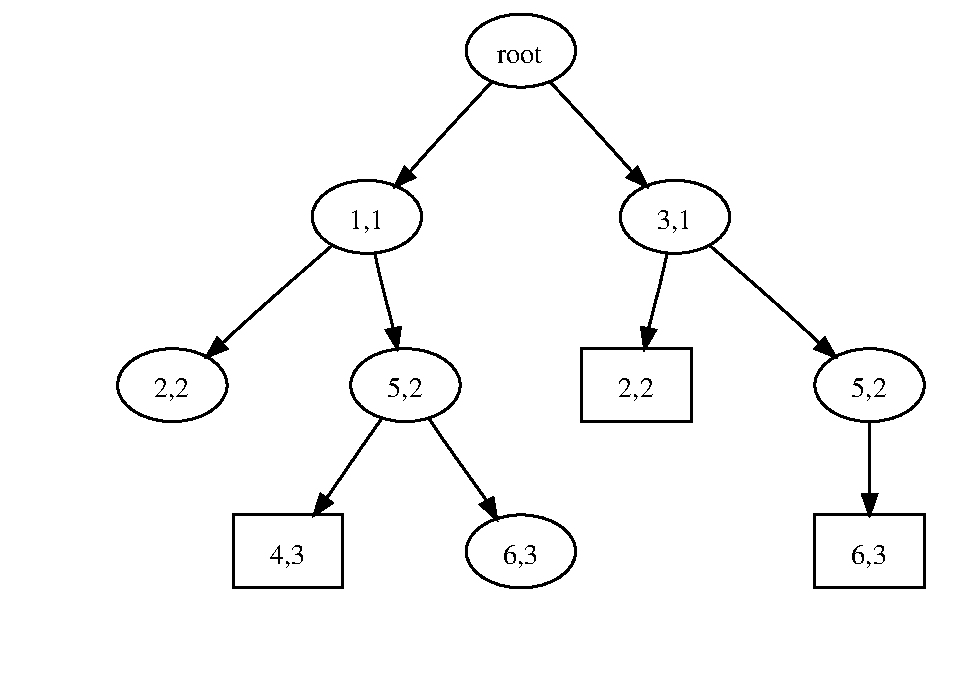
\includegraphics[width=0.85\textwidth]{search-tree-ex.pdf}
	\caption{Algorithm X search tree for the example matrix}
	\label{fig:ex_tree}
\end{figure}

\end{example}

One issue when trying to implement Algorithm X is that the state of the matrix needs to be saved and restored multiple times during the backtrack process.
Each time the algorithm returns the old state must be restored before another path can be explored.
Searching through the matrix to find the non-zero elements is also very time consuming if the matrix is stored as a two dimensional array.
To solve these problems the Dancing Links algorithm was introduced.



\section{Dancing Links}
\label{dlx}

The Dancing Links (DLX) algorithm is based on Algorithm X, but it contains some significant modifications which makes it more suitable for practical applications.
DLX is based on a simple, yet powerful, technique which allows one to reverse any operation made to a doubly-linked list.
If $x$ represents an element in such a list then $x.left$ and $x.right$ points to the previous and next element respectively.
To remove element $x$ from the list the following two operations are applied:
\begin{equation}
	\label{eq:remove}
	\begin{array}{rcl}
		x.right.left &\leftarrow& x.left \\
		x.left.right &\leftarrow& x.right \\
	\end{array}
\end{equation}

Applying these two operations to the linked list in Figure \ref{fig:linked} results in the list in Figure \ref{fig:linked_del}.
These operations modify the links pointing to element $x$ so that an iteration through the list will no longer traverse through this element, but instead skip right past it.
\begin{figure}[htbp]
	\centering 
	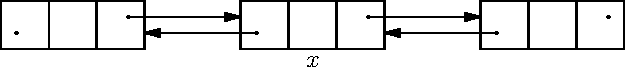
\includegraphics[width=0.8\textwidth]{doubly-linked-list.pdf}
	\caption{Doubly-linked list}
	\label{fig:linked}
\end{figure}
\begin{figure}[htbp]
	\centering 
	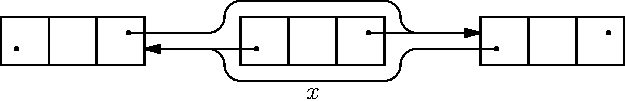
\includegraphics[width=0.8\textwidth]{doubly-linked-list-del.pdf}
	\caption{Doubly-linked list with element $x$ removed}
	\label{fig:linked_del}
\end{figure}

When programming one might be tempted to set $x.left$ and $x.right$ to a null value and delete the $x$ object or let the garbage collector do its thing.
However, smart as that might seem it would prevent one from applying a second set of operations.
In \cite{Hitotumatu79} Hitotumatu and Noshita introduced a pair of operations which allows one to insert an element back into the list in exactly the same place it was removed from.
The following two operations work as the inverse of the operations in (\ref{eq:remove}) by adding $x$ back into the list.
\begin{equation}
	\label{eq:add}
	\begin{array}{rcl}
		x.right.left &\leftarrow& x \\
		x.left.right &\leftarrow& x \\
	\end{array}
\end{equation}

To maintain the state information for the matrix the DLX algorithm uses the operations in (\ref{eq:remove}) and (\ref{eq:add}).
The $x$ element is preserved so that the algorithm can reverse the remove operations, which are used to reduce the matrix.


\subsection{Data structure}
\label{dlx_struct}

DLX stores the matrix as a collection of several circular doubly-linked lists where each non-zero value in the matrix is an element in the lists.
Using this sparse matrix representation saves a lot of memory because the number of zero elements usually outnumber the non-zero elements.
This advantage will normally grow when the size of the matrix increases.
As an example the $n$-queens problem for $n=10$ has 396 non-zero elements, but they only account for 7.33\% of the total number of elements.
% TODO Add density graph/table

Each row and column in the matrix is represented by a separate list.
In addition the set of column headers is also stored in a list.
Each element $x$ in the linked lists have six attributes: $x.left$, $x.right$, $x.up$, $x.down$, $x.column$ and $x.row$.
The $x.row$ attribute is an addition to Knuth's original algorithm to enable detection of the row number.
The first four attributes contains a pointer to an element in the respective list.
$x.left$ and $x.right$ belongs to a row list and $x.up$ and $x.down$ belongs to a column list.
$x.column$ is a pointer to the column header and $x.row$ is a non-negative integer storing the row number of the element.
A column header $c$ has the additional $c.name$ (column name/number) and $c.size$ (number of elements in column) attributes.
Secondary column headers used by the generalized cover problem have their $c.left$ and $c.right$ attributes pointing to $c$ (itself).
The special column header element $h$ acts as a root element for the rest of the data structure.

Figure \ref{fig:matrix_links} shows shows how the matrix in (\ref{eq:cover_example}) can be represented using this data structure.
To avoid clutter the $x.column$ links pointing to the column headers are not displayed in the figure.
\begin{figure}[htbp]
	\centering
	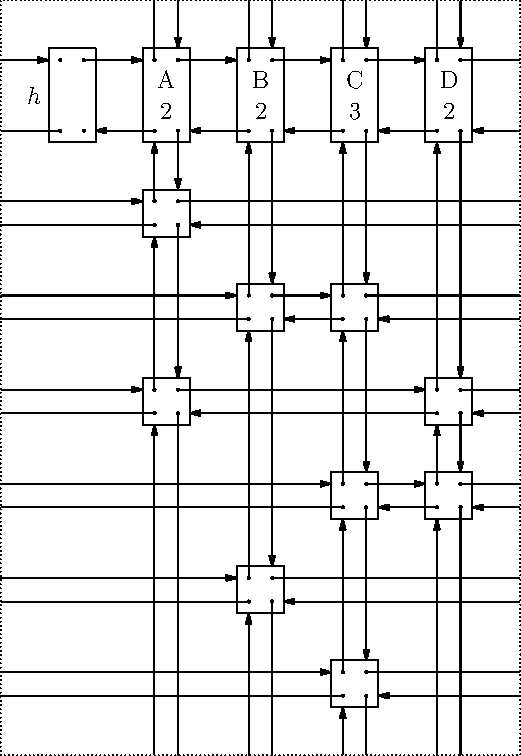
\includegraphics[width=0.52\textwidth]{matrix-links.pdf}
	\caption{Sparse boolean matrix circular quad-linked list representation of the example matrix}
	\label{fig:matrix_links}
\end{figure}


\subsection{Algorithm}

The DLX algorithm is very similar in nature to Algorithm X and in essence the two algorithms work exactly in the same way.
Given the example matrix (\ref{eq:cover_example}) the DLX algorithm will follow the same path as shown in Figure \ref{fig:ex_tree}.
The difference is that DLX uses a specialized data structure together with the linked list remove and add operations to save and restore the state of the matrix.
Comparing Algorithm \ref{alg:algox} and Algorithm \ref{alg:search} reveals that they are very similar in nature.

The DLX algorithm is initially called with $k = 0$ (recursion level 0) and a pointer to the column header $h$ of the matrix.
Printing a solution using the $x.row$ attribute is done by printing $O_{i}.row$ for all $i \in \{1, 2, \ldots, k\}$.
Column selection is done using the $S$ heuristic, which picks the column with the lowest value for $c.size$.
Algorithm \ref{alg:column} simply steps through each column header looking for the lowest size.

\begin{algorithm}[htbp]
	\caption{Dancing Links recursive search.}
	\label{alg:search}
	\begin{distribalgo}[1]
		\PROCEDURE{search($k$)}
			\IF{$h.right = h$}
				\STATE Print solution and return.  \COMMENT{Base case for the recursion}
			\ENDIF
			\STATE $c \leftarrow$ choose\_column()
			\STATE cover($c$)
			\FOREACH{$r \leftarrow c.down, c.down.down, \ldots,$ \textbf{while} $r \neq c$}
				\STATE $O_k \leftarrow r$  \COMMENT{Add $r$ to partial solution}
				\FOREACH{$j \leftarrow r.right, r.right.right, \ldots,$ \textbf{while} $j \neq r$}
					\STATE cover($j.column$)
				\ENDFOR
				\STATE search($k + 1$)
				\FOREACH{$j \leftarrow r.left, r.left.left, \ldots,$ \textbf{while} $j \neq r$}
					\STATE uncover($j.column$)
				\ENDFOR
			\ENDFOR
			\STATE uncover($c$)
		\ENDPROC
	\end{distribalgo}
\end{algorithm}

\begin{algorithm}[htbp]
	\caption{Column selection using the $S$ heuristic.}
	\label{alg:column}
	\begin{distribalgo}[1]
		\FUNCTION{choose\_column()}
			\STATE $s \leftarrow \infty$
			\FOREACH{$j \leftarrow h.right, h.right.right, \ldots,$ \textbf{while} $j \neq h$}
				\IF{$j.size < s$}
					\STATE $c \leftarrow j$
					\STATE $s \leftarrow j.size$
				\ENDIF
			\ENDFOR
			\RETURN{column $c$}
		\ENDFUNC
	\end{distribalgo}
\end{algorithm}

The cover($c$) and uncover($c$) algorithms are the main differences between DLX and Algorithm X.
The purpose of cover($c$) is to remove column $c$ from the column header list and to resolve any conflicts in the column.
It uses the operations in (\ref{eq:remove}) to remove the conflicting elements from the column lists.
The cover($c$) algorithm also increments the value of $updates$ which is used to measure how many operations the search algorithm requires to complete.
One update equals four link modifications or one application of both the linked list remove and add operations.
The $size$ column header attribute is maintained by both the cover($c$) and uncover($c$) algorithms so that the $S$ heuristic works properly.
Algorithm \ref{alg:cover} contains the pseudo code for the cover procedure.
\begin{algorithm}[htbp]
	\caption{Cover column $c$.}
	\label{alg:cover}
	\begin{distribalgo}[1]
		\PROCEDURE{cover($c$)}
			\STATE $c.right.left \leftarrow c.left$  \COMMENT{Remove column $c$}
			\STATE $c.left.right \leftarrow c.right$
			\FOREACH{$i \leftarrow c.down, c.down.down, \ldots,$ \textbf{while} $i \neq c$}
				\FOREACH{$j \leftarrow i.right, i.right.right, \ldots,$ \textbf{while} $j \neq i$}
					\STATE $j.down.up \leftarrow j.up$  \COMMENT{Remove element $j$}
					\STATE $j.up.down \leftarrow j.down$
					\STATE $j.column.size \leftarrow j.column.size - 1$
					\STATE $updates \leftarrow updates + 1$
				\ENDFOR
			\ENDFOR
		\ENDPROC
	\end{distribalgo}
\end{algorithm}

The uncover($c$) algorithm restores the state of the matrix using the operations in (\ref{eq:add}).
Notice that Algorithm \ref{alg:uncover} walks up and left in the lists while Algorithm \ref{alg:cover} walks down and right.
This ensures that the elements are put back in the reverse order in which they were removed.
This is the only way to make sure that all the links are restored to their original state.
\begin{algorithm}[htbp]
	\caption{Uncover column $c$.}
	\label{alg:uncover}
	\begin{distribalgo}[1]
		\PROCEDURE{uncover($c$)}
			\FOREACH{$i \leftarrow c.up, c.up.up \ldots,$ \textbf{while} $i \neq c$}
				\FOREACH{$j \leftarrow i.left, i.left.lseft, \ldots,$ \textbf{while} $j \neq i$}
					\STATE $j.column.size \leftarrow j.column.size + 1$
					\STATE $j.down.up \leftarrow j$  \COMMENT{Add element $j$}
					\STATE $j.up.down \leftarrow j$
				\ENDFOR
			\ENDFOR
			\STATE $c.right.left \leftarrow c$  \COMMENT{Add column $c$}
			\STATE $c.left.right \leftarrow c$
		\ENDPROC
	\end{distribalgo}
\end{algorithm}



\section{Parallel Dancing Links}

To be able to solve more complex exact cover problems the solution process must be distributed to a larger number of computers.
To accomplish this we must first break the problem into smaller pieces.
In \cite{maus-prp} Maus and Aas investigates recursive procedures as the unit for parallelizing.
They introduce some techniques on how to split the recursion tree which can be directly applied to the search tree in DLX.
The main idea is that the algorithm is first run in a breath-first mode so that the search tree is explored one level at a time.
When a certain number of nodes in the tree has been discovered the search stops and the nodes are distributed to a set of computers and solved in parallel.

The search procedure of DLX is a backtrack algorithm which explores the search tree depth-first.
Making this a breath-first algorithm can be achieved by not allowing it to proceed deeper than a certain level in the search tree.
When the given level is reached the partial solution $O$ is saved.
$O$ can then be used to initialize a separate process by running DLX on a different computer (or another processor on the same computer).
As long as the predefined depth $d$ is not too deep or shallow the partial solutions can be used to efficiently solve the exact cover problem in a distributed manner.
If $d$ is too deep (high) the algorithm will find all solutions before the splitting happens, and if it is too shallow (low) the number of partial solutions might be too low to be of any use.
Adding line 10 to 12 in Algorithm \ref{alg:psearch} is the only changes required to make the original Algorithm \ref{alg:search} support this scheme.
\begin{algorithm}[htbp]
	\caption{Dancing Links parallel recursive splitter.}
	\label{alg:psearch}
	\begin{distribalgo}[1]
		\PROCEDURE{psearch($k, d$)}
			\IF{$h.right = h$}
				\STATE Print solution and return.  \COMMENT{Base case for the recursion}
			\ENDIF
			\STATE $c \leftarrow$ choose\_column()
			\STATE cover($c$)
			\FOREACH{$r \leftarrow c.down, c.down.down, \ldots,$ \textbf{while} $r \neq c$}
				\STATE $O_k \leftarrow r$  \COMMENT{Add $r$ to partial solution}
				\FOREACH{$j \leftarrow r.right, r.right.right, \ldots,$ \textbf{while} $j \neq r$}
					\STATE cover($j.column$)
				\ENDFOR
				\IF{$k \geq d$ and $h.right \neq h$}
					\STATE Print partial solution.  \COMMENT{Prevent further recursion}
				\ELSE
					\STATE psearch($k + 1$)
				\ENDIF
				\FOREACH{$j \leftarrow r.left, r.left.left, \ldots,$ \textbf{while} $j \neq r$}
					\STATE uncover($j.column$)
				\ENDFOR
			\ENDFOR
			\STATE uncover($c$)
		\ENDPROC
	\end{distribalgo}
\end{algorithm}

Each partial solution produced by psearch($k, d$) can be used as an initialization vector for the modified search procedure search\_init($O$) in Algorithm \ref{algo:isearch}.
$O$ is the initialization vector and $O.size$ is the length of the vector (number of rows in the partial solution).
The initialization vectors and the matrix can be distributed and the modified search procedure can be run in parallel on each computer.
If required each computer can do further splitting locally to take advantage of multiple processors.
\begin{algorithm}[htbp]
	\caption{Dancing Links search initialization.}
	\label{algo:isearch}
	\begin{distribalgo}[1]
		\PROCEDURE{search\_init($O$)}
			\FOR{$k \leftarrow 0$ \textbf{to} $O.size - 1$}
				\STATE $c \leftarrow$ choose\_column()
				\STATE cover($c$)
				\STATE $r \leftarrow O_k$
				\FOREACH{$j \leftarrow r.right, r.right.right, \ldots,$ \textbf{while} $j \neq r$}
					\STATE cover($j.column$)
				\ENDFOR
			\ENDFOR
			\STATE search($O.size$)  \COMMENT{Do actual search}
		\ENDPROC
	\end{distribalgo}
\end{algorithm}

This approach does not guarantee that each initialization vector provides the same amount of work.
Unfortunately there is no straight forward method to estimate the complexity of the subtree given by a specific initialization vector.
In \cite{knuth75backtracking} Knuth uses a Monte Carlo approach to estimate the running time of a backtrack algorithm.
By doing random walks in the subtree he is able to estimate the cost of backtracking.
This approach would be worth investigating for a future version of DECS.